\chapter{Methods}
\label{methods}

To summarise, the overall approach for determining board state is to first segment each square of the board from the image,
and use those subimages as input to a piece classifier from which the output can be concatenated into a view of the whole board.
Splitting the input to a classifier up by square is a unanimous decision taken by previous authors discussed in \nameref{research} 
as it reduces the problem to a simple classification problem of only piece type and can take advantage of the thoroughly researched area 
of chessboard detection.

\section{Data Collection}
At the heart of any machine learning project is the data.  
It is as important, often more important, than the code and presents many interesting
challenges.  **Why is this?**
Discussed in the following sections are some of the challenges and decisions that were considered.

\subsection{Sensors}
The eminent challenge is acquiring data in the first place and is highly context dependant,

For vision there are a range of sensors we can use to gather data from the real world.
Sensor choice is an important choice for any robotics application as there are 
important tradeoffs, as with any engineering challenge, which must be considered.

**Outline some of the tradeoffs between spatial sensors**

One important distinction to make is the difference between training and inference.
Requirements at the time of training my differ significantly to the requirements at 
inference.  Processing power, energy supply and realtime operation are some
of the constraints that will have to be met when considering different sensors.

Talk about single camera. 

The sensor used throughout this project is the RealSense SR305 which is a RGB-D camera
using structured and coded light to determine depth, it functions best indoors or in a 
controlled lighting situation.  For the reasons outlined above the RGB camera stream is 
mainly relied upon but there will be some discussion and comparision of piece detection 
with the depth sensor.  

Talk about the generic camera

\subsection{Auto-Labelling}
Talk about using a simulator.

A closely related challenge of acquiring the data is that of labelling it too. 
During \nameref{research} multiple past authors have stated the availability of 
datasets for chess piece recognition is sparse \cite{} with some emphasizing
dataset collection took the large majority of their time \cite{}.
It is also widely known that neural networks scale with the number of examples \cite{}, 
which will be explicitly explored for Chess Vision in \nameref{results}.
This however poses the question: how do we get access to a lot of labelled data 
for chess?

Unlike techniques in \cite{}  **Some examples of other auto labelling techniques**
the approach taken here was to maximize speed of collection and flexibility.

Portable Game Notation (PGN) is a common format for recording chess games as a 
series of moves and are widely available online.  All the PGN files used in the 
project were used from \cite{} which has over one million games.  Utilising this
data not only has the benefit of an abundance of chess games but also that the 
recorded games are real and contain positions more likely to appear in game play. 

A program is developed for recording these games with the generic camera interface
as previously described.  The program takes screenshots upon user input (with the
[Enter] shortcut) displaying the move number and image as a result for visual feedback
before saving to disk.  These games can then be automatically labelled using the matching
PGN file.

After the development of this pipeline it was possible to collect over 2,500 \textit{unique} labelled
images in under two hours.

\subsection{Dataset Versioning}
With all this data the next challenge becomes self evident. It is concerned with the question: How do we manage all of this?
As experiments are carried out and iterations on the dataset are performed there will be many changes and variations of the data
that are used to train models.  This is a challenge with data for many reasons, the first being reproducibility.  Say you train a model
that performs really well, then you make some changes in say the balancing of the dataset or even the size and you train again.  If you go 
through a series of changes like this and discover that it performed a lot better the way you had it previously then you might want to roll back.

In typical software engineering a version control system like git \cite{} would be used.  While this is what was used to version the codebase of this project,
there are different challenges with data, namely it's storage.  Code usually takes up megabytes of storage, the Linux Kernel source code for example contains
27.8 million lines and is only around 1GB in size \cite{}.  The data used throughout this project came to >20GB.

There are many proposed solutions for this problem, from managed service like Neptune \cite{} and wandb \cite{}, to self hosted opensource options.  In fact Git has its own
solution called Git Large File Storage (Git LFS) \cite{} which uses the exact same methodology as with code except it will store large files in an external 
remote and only reference those locations in your git repo using a hash of your data's content.  This means if you change any of your data a new copy 
of that data will be stored and it's reference updated.  And so to maintain git's methodology of versioning any change of your data will mean a new copy 
will be stored, rapidly increasing storage costs with changes.  Neptune instead is a more holistic machine learning platform that provides a whole bunch of 
features other than just dataset versioning.  As with other managed services these managed solutions are prone to lock-in and require you modifying your code 
with a bunch of API calls to get them running.
In the end it was found that a custom solution utilising some cloud based object storage proved most useful, with the least amount of effort and cost.  
Perhaps the wide variety of solutions all with different approaches is evidence of this not yet being
a solved problem.  To demonstrate the cost difference, Git LFS per GB cost is \$0.1 a month which is 4 times more expensive
than amazons most expensive rate of \$0.023 per GB.  With optimisations you can get the amazon S3 bucket price down to \$0.0125 making Git LFS 8 times
more expensive.  These numbers may look small but they add up with time and scale, especially when versioning many changes where copies and diffs need
to also be stored.

The solution used in this projects centers around 3 elements: The \textit{Game}, a \textit{Labeller} and the \textit{Storage} facade.  

The storage 
facade's purpose is to abstract file storage so that it could work with any backend and provide a simple to use interface for fetching files using a file system.
\verb|file = open(Storage("img.png"))| 
for example will give you the file descriptor for img.png cached from the filesystem if it exists, pulling it from an external store if not.  
This was very useful for training across different VMs in the cloud and could work with any storage implementation.
The only backend implemented was Amazon S3 bucket store, and used less than 50 lines of code.

The Game class \ref{} is how chess data specifically is managed.  Each instance of Game represents one 'unit' of data where each unit is a recorded chess game.
You can record a game by using the recorder application described in the autolabelling section and is simply a sequence of images with
an associating PGN description. \textit{LabelOptions} can be set on a game which will be used by a Labeller to describe exactly how the autolabeller 
should function.  For example, \verb|Game("Kasparov", LabelOptions(margin=50))| will create a game that should be labelled
with a margin of 50px surrounding each square.  As will be discussed later it is this game object that will version the data used to train a model while dramatically
decreasing the storage cost.  This is opposed to storing a new entire labelled dataset everytime a slight change is made, i.e chaning the margin of each square.

As different model architectures were explored, different labelled data was need entirely.  For example, one model may only be 
predicting whether a piece is a black or white pieces whereas another may be prediting the type of piece.  To cater for this variance while keeping the rest of the 
training pipeline unchanged the Labeller abstraction is used.  Each labeller has a function that can take in a Game and output a series of X, Y input, target pairs.
These can then be saved to disk for the \textit{ChessFolder} pytorch dataset to handle. 
This could even be extended to more complicated labels like bounding boxes or multiple input images.

One important note in implementation is the use of python generators which dramatically reduce memory usage and speed up the auto-labelling pipeline by over 10 fold in 
places.

\section{The Model}
Given this data what is are model meant to do.

\subsection{Experiment Tracking}
Over 500 hours was spent on training models with many different architectures each trained hundreds of times
on slightly varied hyperparameters.  This makes the processes which is commonly refered to as Experiment Tracking a very important one.
It would be good to visualise all these experiemnts and be able to roll back to old models.  As with dataset versioning there are a plethora of 
new managed services that promise they can do this for you.
The appoach opted for during this project utilised an opensource solution called Guild \cite{}.  The main reason for this choice was beacause of 
it's unopinionated manor, requiring zero code changes.  GuildAI leverages the filesystem to save \textit{runs} including the environment configuration
at the time of training.  A run is made from the command line and
represents one iteration of a model \verb|guild run train --remote ec2 EPOCHS=10 LR=0.001| and can even be executed remotely via ssh to give easy access to 
GPU machines.  It can also perform hyperparameter optimization using built in techniques like grid search, random search, gradient boosted regression trees 
or even your own custom optimizer.  To enable the zero code change promise, guild fetches hyperparameters from a variety of places including globals set within 
your training script, configuration files and commandline arguements.
This method was greatly prefered to using a paid managed service or some other solution which require a database to setup allowing for quick integration and
customization.  The previously mentioned dataset versioning method also greatly benefits from guilds use of the filesystem as within each run we can also store 
the Games and Labeller that was used to train the model. 
TesnorBoard integration also played a huge roll as it provided a easy to use, visual place to interpret and compare runs.  See \autoref{}
for examples.

All in all allowing for easy reproducability and insight into 


\subsection{Board Segmentation}
Aruco markers are chosen for board corner point detection as a very simple method.
With the corner points of the board the perspective transformation is calculated using
Gaussian elimination \cite{gauss}, as demonstrated in \autoref{fig:corner}.
Although Aruco markers require customizing the environment they are very fast at 
inference and allow the focus to remain on piece recognition, from which
\nameref{research} showed is less studied and reliable.  In a more holistic solution the 
iterative heatmap approach proposed in \cite{heatmap} would be recommended.

\begin{figure}[h]
    \centering
    \begin{subfigure}[b]{0.32\textwidth}
        \centering
        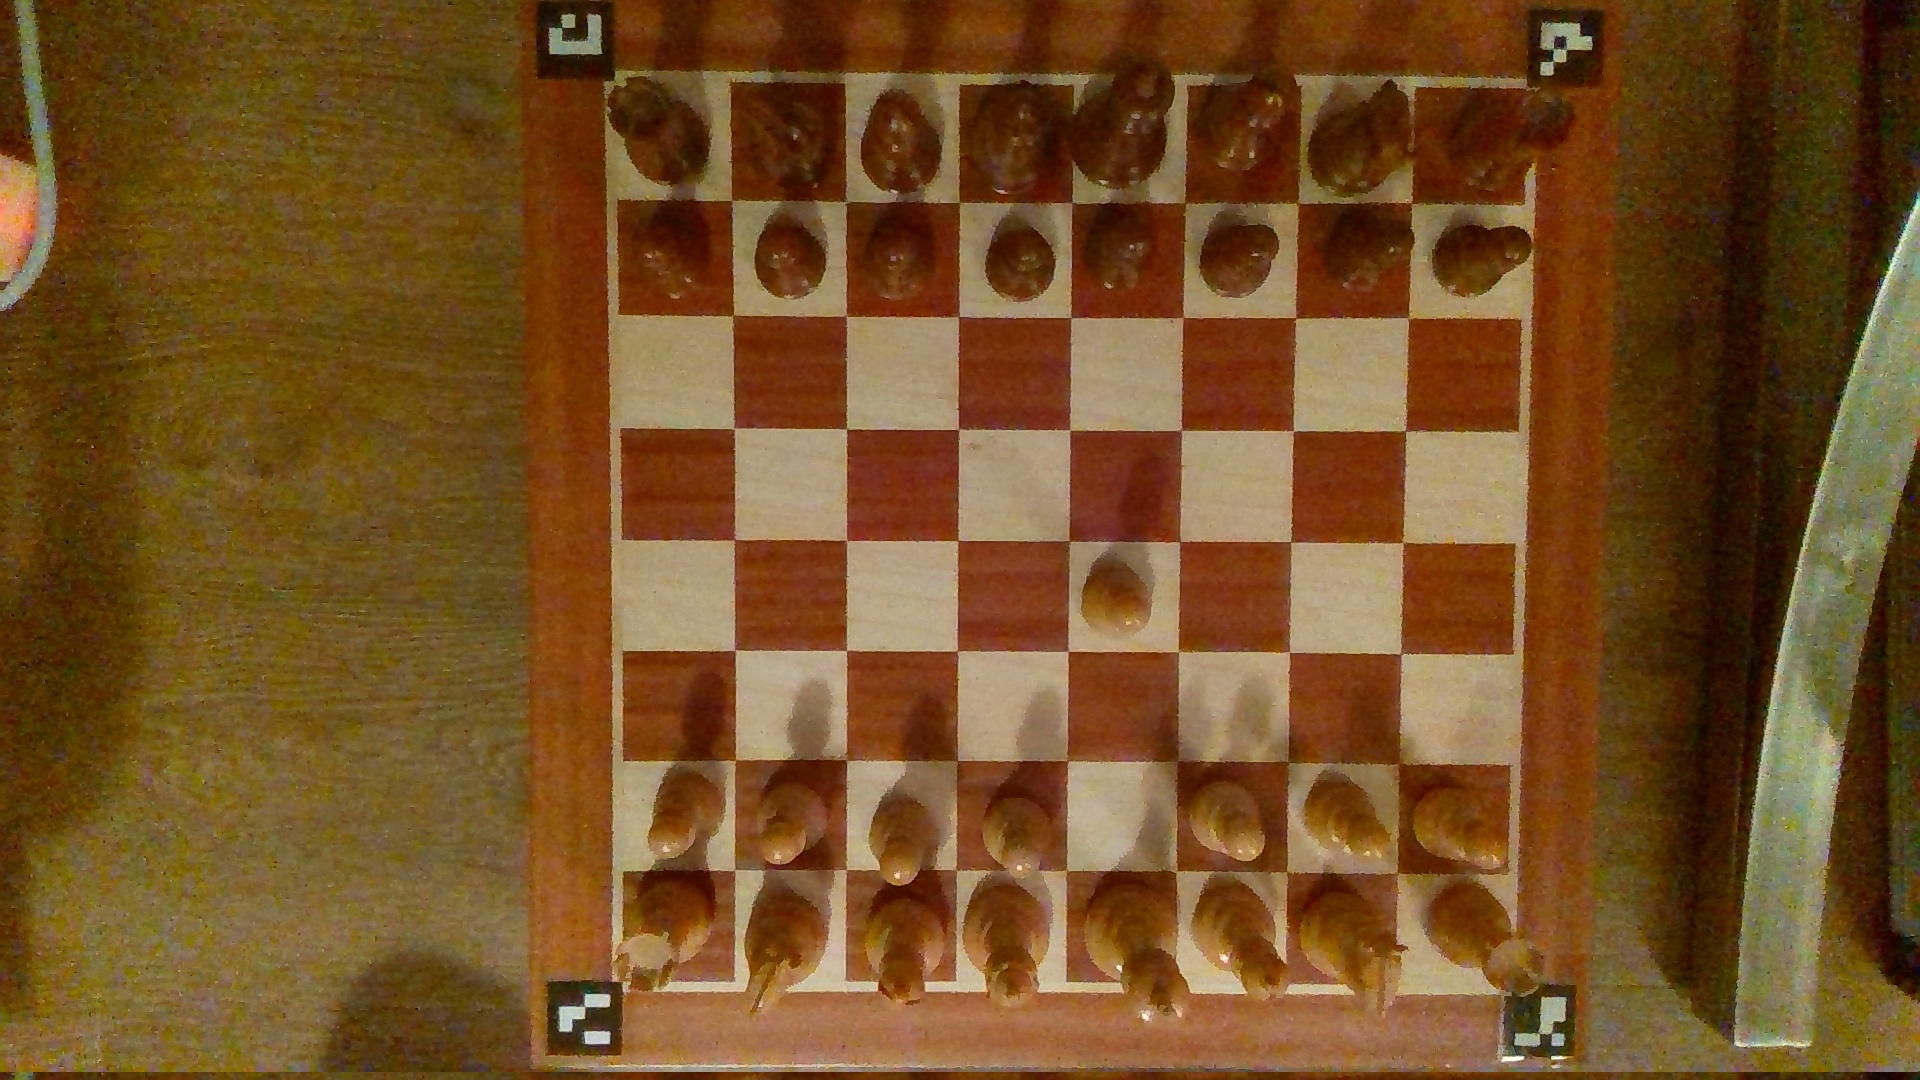
\includegraphics[width=\textwidth]{board.jpg}
        \caption{Original Image}
    \end{subfigure}
    \hfill
    \begin{subfigure}[b]{0.32\textwidth}
        \centering
        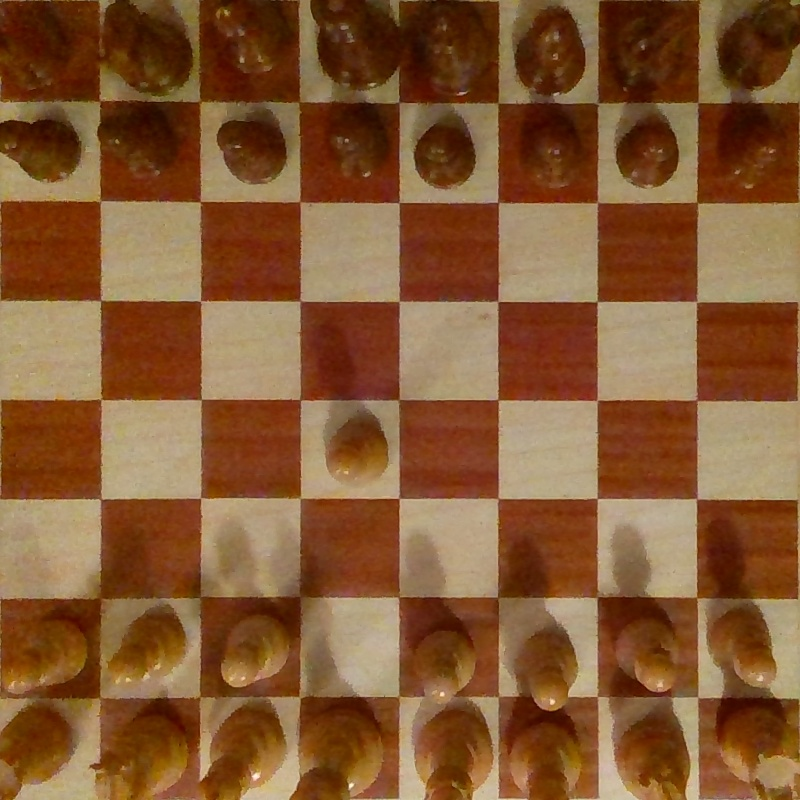
\includegraphics[width=\textwidth]{segmented_board.jpg}
        \caption{Reorthogonalisation}
    \end{subfigure}
    \hfill
    \begin{subfigure}[b]{0.32\textwidth}
        \centering
        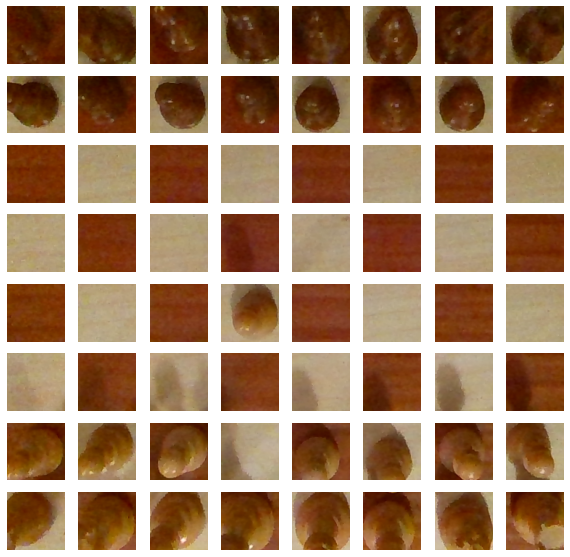
\includegraphics[width=\textwidth]{separated.png}
        \caption{Square Segmentation}
    \end{subfigure}
\caption{Board Squares Segmentation Process}
\label{fig:corner}
\end{figure}
    

\subsection{Piece Recognition}
Now that the board has been segmented including all of it's squares, it is time for the fun stuff.  That is
to determine what piece, if any, occupy each square.  To start, a good baseline is found.  
A good baseline is a simple model to understand and easy to get decent results with.
For classification, the pathological baseline would be a uniformly random model, which could easily be extended to use a categorical distribution.
The probability mass function for a categorical distribution of $k$ categories numerically labelled $0, ..., k$ is

$$ f(x \;|\; \bm{p}) = \prod\limits_{i=0}^{k}{p_i^{[x=i]}} $$

where $\bm{p} = (p_0, ..., p_k)$ and $p_i$ represents the probability of an image of category $k$ being sampled from the training set.
Since $\sum_{k}{p_k} = 1$ you can generate the probabilities by normalising the count of each category in the training set.  Algorithmically 
sampling from the distribution can be done using inversion sampling which requires calculating the cumulative distribution function.

Of course you could just use pytorch \cite{} \verb|Categorical(tensor([0.25, 0.5, 0.25])).sample()|

This is common practice in exploratory machine learning \cite{} so that the transitions
made are always from a known and working state.  It becomes very easy to see if an experiment is not working by comparing it to your baseline and 
makes it easy to go back.

Keeping to this strategy, the Multilayer Perception (MLP) or fully connected network \cite{} was the first neural network to be explored.
We explore nerual network approaches as they have proved most effective for image classification \cite{}, they are also relatively simple to deal
with as no hand-crafted feature extraction is needed and end-to-end solutions are much more viable.
By starting with the MLP, all complexity from the network is stripped away so the more extraneous elements such as the training loop and 
evaluation metrics can be built and tested.

Evaluation metrics were very imporatnt in developing as loss is not that human interpretable.  Firstly accuracy, which is much more interpreatable, 
is calculated to be the ratio of correct classifications to total number of sample images.  This could then be extended to top-n accuracy which 
takes accuracy to be:  

INSERT MATH.

As the number of evaluation metrics grew it became prudent to encapsulate them into an \textit{Interpreter} class so as to not clog up our 
training loop which itself is within a \textit{Trainer} class to encapsulate it's implementation away from the training script which will 
see frequent changes during experimentation.  Some of the first additional methods added to the Interpreter is \verb|plot_top_losses| and
\verb|plot_confusion_matrix| to make it significantly easier to find which classes the model was confusing and which specific images it 
found difficult to classify giving hugely helpful insight into the dataset itself and even finding bugs in the autolabelling pipeline.

Before training, a fixed random seed was important so that it was possible to tell whether or not any particular change was positive since all models started
from the same initalisation.  The initalisation of the final layer was hard coded to be an equal distribution, sensible initalisations of final layer can have 
a noticable effect on training convergence \cite{}.

SHOW PLOTS

Once the full training and evaluation structure is functional, new features can be incrementally added and architectures explored.
 - human labelled dataset?

Another strategy was to purposely overfit models during training.  It was easy to tell when a model was overfitting by splitting the data into
training and validation sets \cite{} and viewing the relative losses in TensorBoard as can be seen in \autoref{}.  The reason for doing this
was that if the model was able to overfit (i.e. achieve $\sim100\%$ accuracy on the training set) then it was able and big enough to learn distinguishing features or
as is sometimes put: the model has sufficient entropic capacity.  It is then a lot easier to make it generalise well, for example by reducing the number of parameters, 
than to go from an underfitting model to a generalised one as you don't necessary know where the problem lies for not fitting to the data.

SHOW overfitting

There are many ways to fight overfitting as typically referered to as regularization techniques, perhaps the easiest of which is early stopping \cite{}.
The way this was implemented in our Trainer was to save the model after the first epoch and consquently after every other epoch for which the validation 
loss was less than the previously saved model.  It is possible to then stop training entirely if after a set number of iterations no improvement is seen 
in the validation loss.

As mentioned in \nameref{research} convolution operations, and in particular differentiable convolutional operations have had monumental 
impact on the field of computer vision and so this was the next experiment. Quite quickly, especially with a limited dataset, overfitting 
became a major problem to overcome and so many experiments were positioned to solve this problem.  Below are an overview of some of those 
experiments including some final optimisations to squeeze as much performance out of our model as possible.


\subsubsection{Architecture}
ConvNext https://arxiv.org/pdf/2201.03545.pdf

Different architectures such as ResNets \cite{}, ConvNext \cite{} and ViT were explored as well.

\subsubsection{Loss Function}
https://towardsdatascience.com/choosing-and-customizing-loss-functions-for-image-processing-a0e4bf665b0a
https://arxiv.org/pdf/2009.13935.pdf proposes SML may be better than cross-entropy

\subsubsection{Optimizer}
An important part of any neural network training loop is the optimiser and so we will explore the effect of swapping these out.

[put into results]
AdamW was found produce more attractive results from comparing SGD with/without momentum and Adam and AdamW \cite{}
Learning Rate, Weight Regularization.

Learning rate scheduler, leave this till the end.

\subsubsection{Batch Normalization}
https://arxiv.org/abs/1502.03167 and renorm for small batch sizes https://arxiv.org/abs/1702.03275

https://arxiv.org/abs/1207.0580 shouldn't be used after convolution layers \cite{} there has been some work https://arxiv.org/abs/1904.03392

Pooling and DropPaths

\subsubsection{Transfer Learning}
There appears to be a trend occuring in the deep learning space.  Some organisation spends millions training an impossibly large nerual network
and others more and more are using these models, often fine-tuning for their own use cases.  \cite{} uses these large models as fixed feature extractors.

This appraoch makes sense as it is inpractical to retrain huge nerual networks that take weeks, millions of dollars and wasteful amounts of energy
to train \cite{}.

In the case of CNNs we can see the features that kernals in the early layers learn \cite{} are often very simple shapes and will be common for all
computer vision tasks.  This will explored this further in the results section as we visualise kernals from both random initalised models and 
pretrained models.

\subsubsection{Multitask Learning}

Consider change to loss function.  Could do a weighted some of losses and then some kind of searcg (grid search) for the best weights.

\subsubsection{Augmentation}
Data augmentation is strategy every machine learning practioner wants to have in their aresonal.  It addresses the data problem, allows us to truly 
leverage the data we have and generalise our models further.  The MINST \cite{} dataset itself was created using data augmentation.
In the case of chess piece classification, the correct augmentations or transformations should be chosen.
Go onto list the transformations used and why.


\section{Recording a Chess Game to PGN}
The goal of this section is to discuss methods for using the proposed piece classifier to record an entire game of chess, played on a real board, 
to a PGN formatted file.

The general approach is to generate a board state at each fetched frame.  That is to segment the board and each of it's squares, send each square 
through a forward pass of the piece classifier described above and finally collate the predictions together into a board state.  A board state is 
a generic term that in actuality could be many things, but in this case it is sufficient enough to think of it as Forsyth-Edwards Notation (FEN).
This board state can then be compared with the previous board state and if any difference is detected then that move is added as a child node.
This tree structure gives flexibility for many variations of the same game to be recorded to later be parsed and encoded to PGN.


\begin{figure}[h]
    \centering
    \begin{subfigure}[b]{0.48\textwidth}
        \centering
        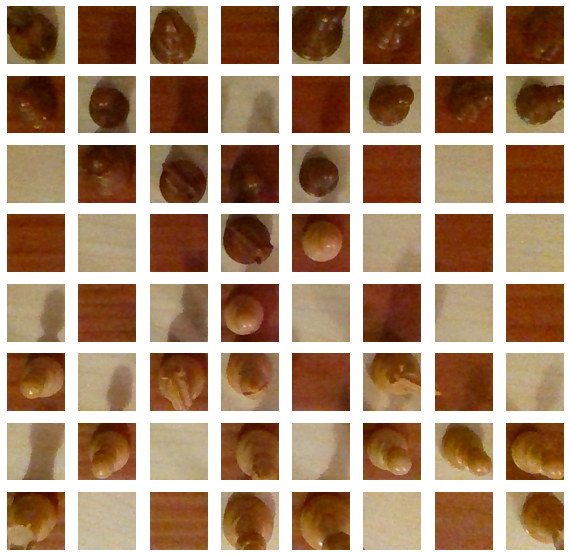
\includegraphics[width=\textwidth]{sample_board.png}
        \caption{Frame after Segmentation}
    \end{subfigure}
    \hfill
    \begin{subfigure}[b]{0.48\textwidth}
        \centering
        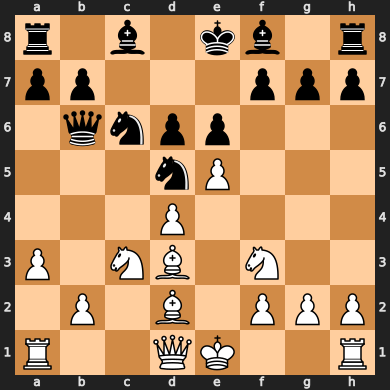
\includegraphics[width=\textwidth]{fen.png}
        \caption{Prediction Vision State}
    \end{subfigure}
% \caption{Board Squares Segmentation Process}
\label{fig:visionstate}
\end{figure}

\subsection{Chess Engines}
As leveraged by others before \cite{} a chess engine and other statistical methods \cite{} can be used to increase the reliability of board state 
prediction when the normal rules of chess can be assumed to be abided by.  The piece classifier described above makes no such assumptions, but as 
the output of this module is a PGN file (which in itself assumes the normal rules of chess??) it is safe to assume them here without loss of 
generality.  In this case leveraging the rules of chess means that we assume the starting state of the board and only allow legal moved to be recorded.

To do this, two concepts are introduced: \textit{VisionState} and \textit{BoardState}.  With some simplification, VisionState is a lightweight 
representation of board as the model sees it in the last fetched frame.  The BoardState starts at a known state and is then only updated if the VisionState at 
any time step represents a legal move from the BoardState. When the BoardState reaches a terminal state or otherwise receives a cancel signal in cases of a 
draw or resignation the game tree is parsed and the PGN saved to disk.

TALK about why

To add even more redundancy the VisionState has a memory of length $N$, where memory is in an average of states over the last $N$ frames.

\subsection{Motion}
One factor that was found to still sometimes break this system was motion.  Moving pieces across squares and hands flailing over the board confused the
model.  Even with the separation of the BoardState and memory to remove anomalous predictions - especially when motion persisted for longer periods.  

In a lot of these situations the actual board state in undefined.  That is because a piece has been lifted and so most now be moved but not yet let go 
and so it's definition may be undetermined.  Because of this is it not unreasonable to halt inference all together.  User input to indicate when a move
has been completed is a common strategy \cite{}, but goes against the purpose of building such a system all together - autonomy.  Instead a motion detector is 
employed.  Even the naive motion detector of using a threshold over the absolute difference between each consecutive frame was found to be sufficient for removing these
disturbances.  Some other methods such as SIFT and SURF were also explored but found to be more computationally expensive that necessary.
